\documentclass[preprint,12pt,authoryear]{elsarticle}
% LISFLOOD-FP 8.4 manuscript for Environmental Modelling & Software.
% Generated by make_ems.py from LISFLOOD_8.4.tex (Copernicus source): the body
% text is identical; only class, front matter and back matter differ.
\usepackage{amsmath,amssymb}
\usepackage{graphicx}
\usepackage{booktabs}
\usepackage{tabularx}
\usepackage{multirow}
\usepackage{xcolor}
\usepackage[T1]{fontenc}
\usepackage{lineno}
\usepackage{url}
\urlstyle{same}
\emergencystretch=3em
\newcommand{\pend}[1]{\textcolor{red}{[#1]}}
\journal{Environmental Modelling \& Software}

\begin{document}
\begin{frontmatter}

\title{LISFLOOD-FP 8.4: portable multi-GPU flood solvers with hydrological losses and optimised pluvial-flood CUDA solvers, validated on real cases and against three other GPU solvers}

\author[lux]{Haseeb ur Rehman\corref{cor1}}
\ead{haseeb.rehman@uni.lu}
\author[lux]{F\'{e}licia Norma Teferle}
\author[shef]{Georges Kesserwani}
\cortext[cor1]{Corresponding author.}
\affiliation[lux]{organization={Department of Engineering, Faculty of Science, Technology and Medicine, University of Luxembourg},
  addressline={6 rue Richard Coudenhove-Kalergi}, postcode={L-1359}, city={Luxembourg}, country={Luxembourg}}
\affiliation[shef]{organization={Department of Civil and Structural Engineering, University of Sheffield},
  addressline={Mappin Street}, postcode={S1 3JD}, city={Sheffield}, country={United Kingdom}}

\begin{abstract}
LISFLOOD-FP 8.4 adds constant-rate, Green--Ampt and Horton infiltration and
evaporation to all seven CUDA solvers and to native Apple Metal FV1, FV2, DG2
and ACC, runs FV1, FV2 and DG2 on several GPUs, and makes CUDA FV1 and ACC
1.3--3.3 times faster than 8.3 with identical predictions. The losses match
analytical solutions within 1\,mm, FV1 is identical on one and four GPUs, and
on four FloodCastBench events the stored water ends within 4.4\,\% of the
references. For the July 2021 pluvial flood of the upper Alzette (4.7 million
cells), CUDA FV1, HiPIMS, SERGHEI-SWE and TRITON ran on the same inputs and
hardware; all overestimate the peaks without infiltration. Uncalibrated
Green--Ampt parameters from European soil databases raise the mean
Nash--Sutcliffe efficiency at four gauges from 0.12 to 0.66 (HiPIMS: 0.71);
Horton gives 0.64. CUDA FV1 is the fastest (33\,min on one A100); four GPUs
give a speed-up of 1.2--1.9.
\end{abstract}

\begin{highlights}
\item Infiltration and evaporation added to all CUDA and native Apple Metal solvers
\item FV1, FV2 and DG2 run on several GPUs; FV1 identical on one and four GPUs
\item CUDA FV1 and ACC steps 1.3--3.3 times faster than in 8.3, identical predictions
\item Uncalibrated Green--Ampt raises mean NSE at four Alzette gauges from 0.12 to 0.66
\item CUDA FV1 fastest of four GPU solvers (HiPIMS, SERGHEI-SWE, TRITON) on the Alzette
\end{highlights}

\begin{keyword}
flood model \sep shallow water \sep GPU \sep infiltration \sep Apple Metal \sep multi-GPU \sep LISFLOOD-FP
\end{keyword}

\end{frontmatter}
\linenumbers

\section{Introduction}\label{sec:intro}

LISFLOOD-FP solves the two-dimensional shallow-water equations with a
local-inertial scheme (ACC; \citealp{BATES201033}), a first-order
finite-volume scheme (FV1), a second-order finite-volume scheme (FV2) and a
second-order discontinuous Galerkin scheme (DG2), with GPU versions of these
solvers and of three variants on non-uniform and adaptive meshes
\citep{Shaw2021,Sharifian2023,Chowdhury2025,LISFLOODFP82zenodo}.
Version 8.3 made the uniform-grid CUDA solvers faster and reproducible and
added an Apple Metal back end for FV1, so that
the July 2021 flood of the upper Alzette (Sect.~\ref{sec:alzette}) could be
simulated competitively on an Apple laptop instead of an NVIDIA A100 of a computer cluster.
The developments of this paper stem from the same application, the
simulation of pluvial floods at catchment scale from rainfall on a 10\,m
grid, and the CUDA FV1 solver that serves it is the solver carried through
the validation of Sect.~\ref{sec:alzette}.

Three limitations remained, and this paper addresses them in turn. First,
infiltration and evaporation were applied only by CPU solvers: a uniform
infiltration rate by the local-inertial solver and a per-cell rate by the
sub-grid channel model, which 8.4 leaves unchanged. The FV1 and DG2
solvers on the CPU and every GPU solver read the loss keywords and ignored
them, so a GPU flood simulation was purely hydraulic. This can be a large
omission in pluvial floods, such as the catchment-scale event simulated in
Sect.~\ref{sec:alzette}, where infiltration removes about one third of the
rain.
Second, on Apple computers FV2, DG2 and ACC ran only on the CPU. Third,
every GPU simulation ran on a single device, which limits the grid size and
the turnaround of large domains.

Version 8.4 adds three infiltration models (a constant rate, Green--Ampt
and Horton) and evaporation to all seven CUDA solvers, ports FV2, DG2 and
ACC to Metal with the same losses, distributes FV1, FV2 and DG2 over
several GPUs (Table~\ref{tab:support}) and makes the CUDA FV1 and ACC
solvers faster. These two are the solvers used for the real events of
Sect.~\ref{sec:validation}: FV1 solves the full shallow-water equations,
which rain-driven flow over steep terrain requires, and ACC is the
local-inertial solver of operational floodplain modelling. While testing the
losses we also
found and corrected a free outflow boundary that admitted water when the
flow at the edge pointed into the domain. Section~\ref{sec:developments}
describes these developments and their use. Section~\ref{sec:verification}
verifies them against analytical solutions, against the previous release
and across back ends and GPU counts. Section~\ref{sec:validation} evaluates
the accelerated CUDA ACC and FV1 solvers on large real pluvial floods: first
the hydraulics, against the reference simulations of the FloodCastBench
dataset \citep{Xu2025floodcastbench}, and then the infiltration models, with
CUDA FV1 alone, for the July 2021 flood of the upper Alzette, against observed
discharge and against three independent GPU solvers run on the same inputs
and hardware: HiPIMS \citep{Xia2019hipims}, SERGHEI-SWE
\citep{CaviedesVoullieme2023serghei} and TRITON
\citep{MoralesHernandez2021triton}. All three are, like FV1, first-order
finite-volume solvers written in CUDA, so the comparison is like for like and
isolates the loss models from the hydraulic scheme.
Section~\ref{sec:performance} reports the computational cost and the hardware
limits of the solver, and Sect.~\ref{sec:limits} states what remains
unfinished.

\begin{table}[t]
\caption{GPU capabilities added in 8.4. ``Losses'' denotes constant-rate
(uniform or gridded), Green--Ampt or Horton infiltration, each with optional
evaporation. Metal was absent in 8.2; in 8.3 it provided FV1 without losses.
Dense modes run the Metal FV1, DG2 or ACC operator on every cell of the
finest grid and provide no adaptive mesh.}
\label{tab:support}
\centering\small
\begin{tabularx}{\textwidth}{@{}l>{\raggedright\arraybackslash}X>{\raggedright\arraybackslash}X>{\raggedright\arraybackslash}X@{}}
\toprule
GPU solver & CUDA in 8.4 & Metal in 8.4 & Several GPUs in 8.4 \\
\midrule
FV1 & losses added & native (from 8.3); losses added & CUDA and Metal \\
FV2 & losses added & new native solver with losses & CUDA and Metal$^{a}$ \\
DG2 & losses added & new native solver with losses & CUDA and Metal$^{a}$ \\
ACC & losses added & new native solver with losses & no \\
ACC\_NUGRID & non-uniform mesh; losses added & dense ACC mode with losses & no \\
HWFV1 & adaptive mesh; losses added & dense FV1 mode with losses & no \\
MWDG2 & adaptive mesh; losses added & dense DG2 mode with losses & no \\
\bottomrule
\end{tabularx}
\\[2pt]{\footnotesize $^{a}$ Scaling not yet measured; on Metal all ranks share one GPU (Sect.~\ref{sec:limits}).}
\end{table}

\section{Developments in version 8.4}\label{sec:developments}

\subsection{Infiltration and evaporation on the GPU}\label{sec:losses}

The losses are evaluated cell by cell on the GPU once per time step: after
the hydraulic update in FV1, FV2 and DG2, and, in ACC, at the point where the
CPU ACC solver applies them (after the dry check and before the depth
update). Cells without data are skipped. One infiltration model is chosen in
the parameter file; evaporation, a time series in mm\,day$^{-1}$ that is
uniform in space as in the CPU solvers, can be combined with any of them.
Every parameter of the three infiltration models is either a number or a grid
file.

\paragraph{Constant rate} As in the CPU solvers, every cell whose water
depth exceeds the drying threshold (keyword \texttt{depththresh}, 1\,mm by
default, below which a cell is treated as dry) loses $(i + e)\,\Delta t$, where $i$ is the infiltration rate
(keyword \texttt{infiltration} in m\,s$^{-1}$, or a grid
\texttt{infilfile} in mm\,h$^{-1}$), $e$ the evaporation rate and $\Delta t$ the time step. The
water depth never falls below zero.

\paragraph{Green--Ampt} A cell with water infiltrates at
\begin{equation}
f = K_s\left(1 + \frac{(\psi + h_0)\,\Delta\theta}{F}\right),
\end{equation}
where $K_s$ is the saturated hydraulic conductivity, $\psi$ the soil suction
head at the wetting front, $\Delta\theta$ the soil capacity (porosity minus
initial moisture content), $h_0$ the depth of ponded water and $F$ the
cumulative infiltration \citep{GreenAmpt1911,MeinLarson1973}; these are the
parameters of the model as used in flood modelling software such as TUFLOW
\citep{TUFLOW2025}. The increment over a time step, $\Delta F = F' - F$, is
calculated from the implicit Euler step $F' = F + k\,(1 + M/F')$, with
$k = K_s\Delta t$ and $M = (\psi + h_0)\Delta\theta$, which has the closed
form $F' = \tfrac12\big((F + k) + \sqrt{(F + k)^2 + 4kM}\big)$. The increment
may not exceed the water in the cell nor, if a soil depth $D$ is given, the
storage that remains in the soil, $D\,\Delta\theta - F$.

\paragraph{Horton} Horton's infiltration capacity decays from an initial
rate $f_0$ to a final rate $f_c$ with a rate constant $k_H$
\citep{Horton1941}. In its original form the decay follows elapsed time, so
the capacity of a cell falls even while the cell is dry. Version 8.4 uses
the cumulative form adopted in the Storm Water Management Model
\citep{RossmanHuber2016}, in which the capacity depends on the depth already
infiltrated: the cell is assigned the equivalent time $t_e$, the time under
continuous ponding at which the cumulative infiltration would reach its $F$,
from
\begin{equation}
F = f_c\,t_e + \frac{f_0 - f_c}{k_H}\left(1 - \exp(-k_H t_e)\right),
\end{equation}
solved by Newton iteration, and may take up to
$F(t_e + \Delta t) - F(t_e)$ of the water present in the time step. Under
continuous ponding this reproduces the classical Horton curve exactly, and a
cell that receives no water keeps its capacity. Green--Ampt and Horton
therefore share the same state, the cumulative infiltration $F$, and the same
treatment of drying; in neither does the soil drain and regain capacity
between rain events, as the recovery option of SWMM allows.

\paragraph{Single precision} The single-precision builds store the water
depth in 32-bit floats, and the loss per time step is often close to the
resolution of the depth (a few micrometres on metres of water). On both back
ends, each cell therefore carries the part of its loss that rounding
discarded to its next time step: the depth after the loss is subtracted from
the depth before it, a difference that is exact by Sterbenz's lemma, and the
shortfall against the intended loss is added to the next step (compensated
subtraction, \citealp{Kahan1965}). The cumulative infiltration $F$ needs more
precision than the depth, because it grows over the whole simulation by
increments that stay small. CUDA stores $F$ as a 64-bit double, which NVIDIA
GPUs support in every build. Apple GPUs have no double precision, so Metal
stores $F$ as a pair of floats updated with an exact two-sum
\citep{Dekker1971} and computes the Green--Ampt increment without the
cancellation in $F' - F$:
\begin{equation}
\Delta F = \begin{cases}
\tfrac12\big((k - F) + \sqrt{S}\big), & F \le k,\\[2pt]
\dfrac{2\,(Fk + kM)}{\sqrt{S} + F - k}, & F > k,
\end{cases}
\qquad S = (F + k)^2 + 4kM.
\end{equation}

\paragraph{Application in each solver} The loss changes the stored
variables of each solver in the way that keeps its flow velocity: FV1 scales
its discharges with the depth; ACC changes only the depth, because its
discharges are stored on the cell faces; FV2 and DG2 lower the mean depth,
keep the depth slopes, so that a flat water surface stays flat, and scale the
discharge coefficients, and a cell whose face would become dry is reduced to
first order. Whatever the solver, the volume removed is summed on the GPU
and reported in the \texttt{.mass} file, whose budget now closes on every
CUDA and Metal solver on one rank (Sect.~\ref{sec:limits}): it counts the
rainfall, sums the stored volume over the cells with data only and reports
the cumulative rainfall minus losses in its last column.

\paragraph{Adaptive and non-uniform meshes} The CUDA MWDG2 and HWFV1
solvers change their mesh every step, and ACC\_NUGRID uses cells of several
sizes. Their soil parameters and state ($F$ and the rounding residual) are
kept on the finest grid, so they persist when cells merge or split. An
active cell evaluates the loss for each of its valid finest children, with
that child's parameters and state, at the active cell's mean depth, and
removes the mean of the resulting losses. Parameters are thus never averaged
before they enter the nonlinear infiltration models, and the \texttt{.mass}
budget above applies unchanged.

\subsection{Free boundary restricted to outflow}\label{sec:free}

A \texttt{FREE} boundary is intended to let water leave the domain. In the
CPU FV1 and DG2 solvers and in the CUDA and Metal FV1, FV2 and DG2 solvers,
the ghost cell of a free boundary copied the state of the adjacent cell,
including its velocity. Where the flow at the edge pointed into the domain,
the boundary therefore supplied water. Version 8.4 reflects the inward
normal component of the discharge in the ghost cell, so that the boundary
passes outflow only; the CPU FV1 ghost cell keeps its tangential component.
The
local-inertial solvers keep their own free boundary, in which the outflow
follows a friction law with the local or a prescribed water-surface slope.

\subsection{Native Metal solvers}\label{sec:metal}

Version 8.4 adds native uniform-grid FV2, DG2 and ACC solvers to Metal and
applies the loss models of Sect.~\ref{sec:losses} to them and to FV1
(Table~\ref{tab:design}). The FV2 and DG2 kernels are ports of the CUDA
solvers; the ACC kernels follow the CPU ACC solver. Three design choices
determine their correctness. First, FV2 adopts the states of the ghost cells
and the step order of CUDA, which a fixed-discharge inflow requires for the
boundary to conserve water. Second, as for FV1 in 8.3, each
face flux is computed once and shared by its two cells, and the kernels are
compiled without the fast-math option, so every run repeats bit for bit.
Third, CUDA DG2 limits the slopes in place, so that a cell may read the slope
of a neighbour before or after it is limited; Metal writes the limited slopes
to a separate buffer and has no such race.

The keywords \texttt{ACC\_NUGRID}, \texttt{HWFV1} and \texttt{MWDG2} select
dense Metal modes that apply the ACC, FV1 or DG2 operator, with losses, on
every cell of the finest grid. A parameter file written for the non-uniform
or adaptive CUDA solvers therefore runs on Apple hardware, but at the memory
and run time of the uniform solver on the finest grid: the non-uniform and
adaptive meshes themselves exist only in CUDA, and porting them was outside
the scope of this release.

\begin{table}[t]
\caption{Native Metal solvers added in 8.4 and their loss implementation.}
\label{tab:design}
\centering\small
\begin{tabularx}{\textwidth}{@{}lX@{}}
\toprule
Solver & Design \\
\midrule
FV2 & port of CUDA FV2: reconstruction, limiter, bed source term and two Runge--Kutta stages, with the boundary states and step order of CUDA \\
DG2 & port of CUDA DG2: nine coefficients per cell in one buffer of nine planes (Metal allows 31 buffers per kernel), friction at the Gauss points, Krivodonova limiter, slopes of the DEM and the start file \\
ACC & follows the CPU ACC solver; a conservative two-pass limiter for drying cells keeps each face flux shared by its two cells \\
Losses & shared kernels for the four native solvers and the dense modes; the same models as CUDA, with the soil state held as a pair of floats (Sect.~\ref{sec:losses}) \\
\bottomrule
\end{tabularx}
\end{table}

\subsection{Execution on several GPUs}\label{sec:multigpu}

FV1, FV2 and DG2 can run on any number of GPUs of one node, with one rank
of the Message Passing Interface (MPI) per GPU; the runs of this paper use up
to four, the GPUs of one node of the cluster used. The
raster is divided into contiguous bands of rows. Each rank advances its own
rows, exchanges the halo rows that the stencil of the solver requires after
every stage, and takes part in a global reduction of the time step. Output is
gathered on the first rank in a fixed global order, so that results can be
compared directly with a run on one GPU. The same decomposition is used by
Metal, where all ranks share the GPU of the computer; there it serves to
verify the decomposition rather than to accelerate the run. ACC, the
non-uniform \texttt{ACC\_NUGRID} solver and the adaptive \texttt{HWFV1} and
\texttt{MWDG2} solvers run on one GPU and stop with an error message if more
are requested: distributing their meshes over several devices is outside the
scope of this release.

\subsection{Parameter-file keywords}\label{sec:usage}

The new options are keywords in the parameter file; terrain, boundary,
rainfall and output settings are unchanged. A CUDA FV1 simulation on four
GPUs with Horton infiltration and evaporation reads:
\begin{verbatim}
cuda
fv1
GPUs 4
infiltration horton
horton_f0 f0.asc
horton_fc fc.asc
horton_k 2
evaporation evap.dat
\end{verbatim}
Here $f_0$ and $f_c$ are grids in mm\,h$^{-1}$ and $k_H$ a number in
h$^{-1}$. For Green--Ampt, the line \texttt{infiltration greenampt} is
followed by \texttt{greenampt\_ks} (mm\,h$^{-1}$), \texttt{greenampt\_psi}
(mm), \texttt{greenampt\_porosity}, \texttt{greenampt\_theta\_init}
(volumetric fractions) and optionally \texttt{greenampt\_soil\_depth} (m).
A constant rate is given in m\,s$^{-1}$ (\texttt{infiltration 5.6e-7}) or as a
grid in mm\,h$^{-1}$ (\texttt{infilfile}). On Apple Silicon, \texttt{cuda} is
replaced by \texttt{metal}. A run on $N$ GPUs is started with
\texttt{mpirun -np N}, where $N$ equals the value of \texttt{GPUs}.

\section{Verification}\label{sec:verification}

All tests are distributed with the code. They ran on an NVIDIA A100 (CUDA
12.6) and an Apple M1 Max (macOS 27). Besides tests written for 8.4, they use
the test cases of the 8.2 source \citep{LISFLOODFP82zenodo}: three humps
(T01--T03; \citealp{Liang2009,Shirvani2021}), a dam break through an
idealised city (T05; \citealp{SoaresFrazao2008}), the torrential valley flood
of test 5 of the Environment Agency benchmark (T06;
\citealp{NeelzPender2013,Ayog2021}), the fluvial Carlisle 2005 flood (T07, and
T07s for its first 6\,h; \citealp{Horritt2010,Neal2013}),
dynamic rain (T030) and an irregular free boundary (T031).

\subsection{Loss models against analytical solutions}\label{sec:losstests}

Three groups of tests isolate the loss models from the hydraulics
(Table~\ref{tab:losses}, Fig.~\ref{fig:losses}). T012 is the evaporation and
infiltration test of LISFLOOD-FP: a flat basin holding 0.4464\,m of water
loses 3.6\,mm\,day$^{-1}$ to evaporation and $10^{-8}$\,m\,s$^{-1}$ to
infiltration for 100 days, with variants in which the evaporation rises
linearly and in which a wall separates two halves with different rates. The
expected depth is the initial depth minus the sum of rate times step over
the steps each solver took. In the Green--Ampt test, 0.1\,m of water ponds
on dry soil ($K_s = 10$\,mm\,h$^{-1}$, $\psi = 110$\,mm, $\Delta\theta =
0.23$) for 24\,h; the model is compared with the implicit Euler solution for
the steps it took and with the continuous solution. Variants give the
parameters as grids, add a soil depth of 0.2\,m and set $K_s = 0$ on one
half. In the Horton test, 0.2\,m of water ponds in a closed box ($f_0 =
60$\,mm\,h$^{-1}$, $f_c = 10$\,mm\,h$^{-1}$, $k_H = 2$\,h$^{-1}$); the water
never runs out, so the infiltrated depth follows the classical Horton curve
exactly.

\begin{table}[t]
\caption{Loss tests: largest depth error against the expected depth for
FV1\,/\,FV2\,/\,DG2\,/\,ACC on CUDA (A100) and Metal (M1 Max), single
precision. ``Exact'' means within the last written digit (0.001\,mm).}
\label{tab:losses}
\centering\footnotesize\setlength{\tabcolsep}{4pt}
\begin{tabularx}{\textwidth}{@{}>{\raggedright\arraybackslash}X >{\raggedright\arraybackslash}p{0.3\textwidth} >{\raggedright\arraybackslash}p{0.3\textwidth}@{}}
\toprule
Test & CUDA (mm) & Metal (mm) \\
\midrule
T012, constant rate, 50 days (223\,mm lost) & 0.0001 / 0.29 / 0.15 / 0.0000 & 0.0001 / 0.0002 / 0.0002 / 0.0000 \\
T012, evaporation ramp, 100 days (360\,mm) & 0.0004 / 0.27 / 0.26 / 0.0002 & 0.0004 / 0.0005 / 0.0005 / 0.0001 \\
T012, wall, per-cell rate, 50 days & 0.0002 / 0.76 / 0.52 / 0.0001 & 0.0002 / 0.0004 / 0.0004 / 0.0005 \\
Green--Ampt, 24 hourly outputs, against implicit Euler & 0.0002 / 0.0009 / 0.0009 / 0.0004 & 0.0003 / 0.0004 / 0.0004 / 0.0004 \\
Green--Ampt, soil depth 0.2\,m (stops at 46\,mm) & 0.000 / 0.001 / 0.002 / 0.000 & exact \\
Green--Ampt, parameter grids; $K_s = 0$ on one half & identical to numbers; no loss & identical to numbers; no loss \\
Horton, 24 outputs in 2\,h (44.54\,mm infiltrated) & 0.040 / 0.017 / 0.017 / 0.002 & 0.040 / 0.017 / 0.017 / 0.053 \\
Volume removed against depth lost & equal (FV2, DG2: within 0.2\,\%) & equal \\
\bottomrule
\end{tabularx}
\end{table}

All 77 checks on Metal and 76 of the 81 on CUDA pass. The other five
compare against assumptions rather than solutions: four find the
\texttt{.mass} log of 8.4 different from that of 8.3, whose budget it corrects
(the depth grids are identical), and one expects 60\,s steps. The CUDA FV2 and DG2 errors in
T012, about 0.2\,\% of the loss, arise because these solvers store the bed
elevation in single precision as given: at 20\,m the last digit is
1.9\,$\mu$m, about the loss of one step, so per-cell rounding creates small
spurious water-surface slopes. With the bed lowered to 0\,m they are exact
(0.0002\,mm), and Metal, which shifts the bed by its lowest elevation, is
exact on the original test. Because changing this storage would change CUDA
FV2 and DG2 results without the new keywords, 8.4 leaves it as in 8.3. The
difference between the model and the continuous Green--Ampt solution
(Fig.~\ref{fig:losses}b) is the error of implicit Euler: up to 0.47\,mm with
the 60\,s steps that all solvers take except CUDA FV1, and 0.94\,mm with the
steps of 136--607\,s that the Courant condition allows CUDA FV1; against the
discrete solution for the steps taken, the error is below 0.001\,mm. In the
Horton test every solver infiltrates the exact 44.54\,mm after 2\,h to within
0.01\,mm (Fig.~\ref{fig:losses}c, d); the larger intermediate differences of
Metal ACC reflect output written at the end of the step that crosses each
5\,min mark rather than an error of the loss model.

\begin{figure}[tp]
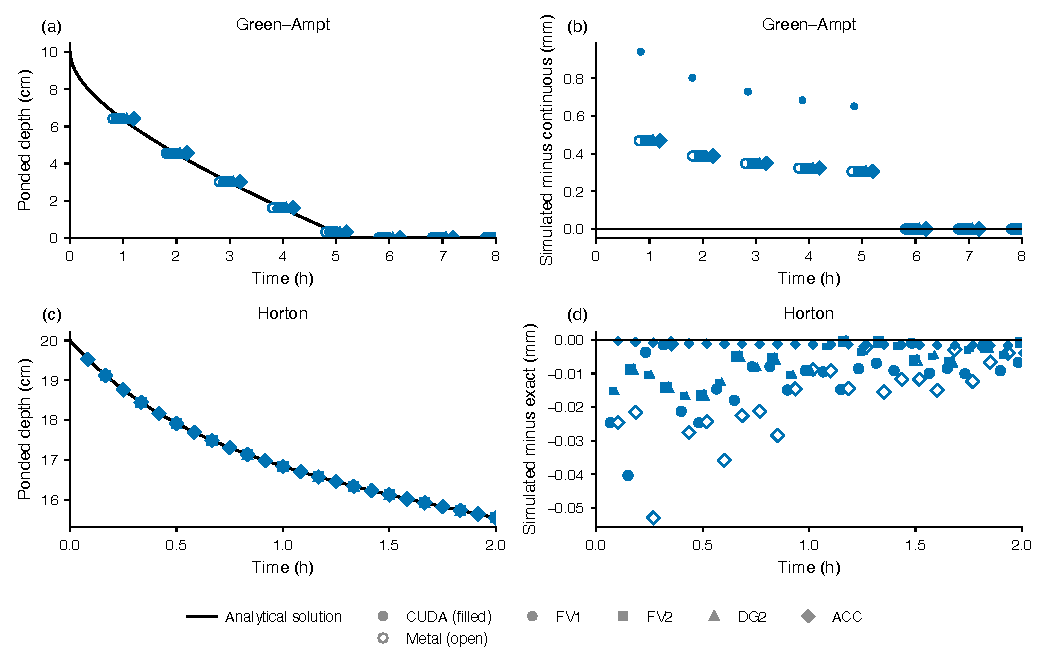
\includegraphics[width=\textwidth]{../figures/f1_losses.pdf}
\caption{Loss models against analytical solutions, single precision.
(a) Ponded depth in the Green--Ampt test and (b) its difference from the
continuous solution at the time each grid was written, which is the error
of implicit Euler (60\,s steps; CUDA FV1 136--607\,s).
(c) Ponded depth in the Horton test and (d) its difference from the exact
solution. Symbols mark the solver, filled symbols CUDA (A100) and open
symbols Metal (M1 Max); in (a) all eight runs coincide in value. In (a), (b)
and (d) the solvers are drawn slightly apart in time so that every symbol
stays visible.}
\label{fig:losses}
\end{figure}

\subsection{Free boundary}\label{sec:freetest}

The boundary correction of Sect.~\ref{sec:free} is tested on a plane that
falls by 2\,\% away from a free western edge towards a closed eastern edge,
with 5\,cm of water at the start and no rain. All flow is directed away from
the free edge, so no water may enter. Before the correction, Metal FV1 and
FV2 gained 0.38\,\% and 0.39\,\% of the initial volume in 30\,min; after it,
FV1 and FV2 conserve the volume to within 0.0003\,\% on CUDA and Metal, and
DG2 to within 0.04\,\%. The
local-inertial and adaptive solvers keep their own rules for the free boundary and are
not affected by the correction.

\subsection{Consistency with version 8.3}

Without the new keywords, 8.4 must reproduce 8.3. On the cases fv1, T01--T03,
T030, T031 and T05, every CUDA solver was run twice with each version before
the boundary correction: every depth grid was identical between the
versions, and the \texttt{.mass} logs differed at most in their last digit,
as between two runs of the same version. The boundary correction changes
results only where the flow at a free edge points into the domain; on the
Alzette case of Sect.~\ref{sec:alzette}, the corrected build reproduces the
hourly discharge of the uncorrected build at every gauge, with and without
infiltration.

\subsection{Losses on adaptive and non-uniform meshes}\label{sec:adaptivetests}

For the adaptive CUDA solvers (MWDG2, HWFV1) and the non-uniform CUDA ACC solver,
analytical basins test constant and per-cell infiltration, evaporation,
drying, Green--Ampt with numbers and grids, the soil-depth limit, raster
orientation, padding and holes without data, and repeated runs. All 218
checks of the adaptive suite, 5 point-source checks and 106 checks of the
non-uniform suite pass. Stored water plus removed volume stays within
$1.2\times10^{-7}$ (adaptive solvers, fixed mesh), $2\times10^{-5}$ (adaptive
solvers, holes without data) and $2.3\times10^{-16}$ (non-uniform ACC) of the
initial volume. On adapting meshes the flow solver itself is not exactly
conservative: the volume drifts by 0.1--1.1\,\% without losses and by
0.2--1.4\,\% with them. These checks complete the verification of the losses
on the non-uniform and adaptive CUDA solvers. The rest of the paper concerns
rain-on-grid simulation of pluvial floods on uniform grids and on several
GPUs, for which these solvers are out of scope: from here on, the solvers
compared are the uniform FV1, FV2, DG2 and ACC on CUDA and Metal.

\subsection{Metal solvers against CUDA and the CPU}\label{sec:metaltests}

Table~\ref{tab:metal} compares Metal FV2 and DG2 with CUDA 8.3, and Metal ACC
with the CPU ACC solver, on the same inputs; the cases contain no inward
flow at a free edge, so CUDA 8.3 and 8.4 give the same reference. Metal FV2
is identical to CUDA on T01, T02 and T031, within 1\,mm on T03 and T030, and
within 1\,cm on 99.9--100\,\% of wet cells of the large cases. Where Metal and CUDA DG2 differ (T03, T05), their first steps agree to
four or five significant digits and the difference grows in these sensitive
cases; CPU and CUDA DG2 differ by as much (44\,\% and 84\,\% of wet cells
identical). ACC is similarly sensitive on T03 and T05, and CUDA ACC is
unstable on T05 (Sect.~\ref{sec:limits}), so the CPU solver is its reference.
On T06, Metal ACC is closer to the CPU solver than CUDA ACC is (75\,\% of
wet cells identical, against 42\,\% for CUDA). Every Metal run repeats bit
for bit. Of the four uniform solvers, FV1 is the one whose Metal port was
already compared with CUDA in 8.3, that passes every loss test of
Sect.~\ref{sec:losstests} on both back ends, and that runs on several GPUs on
both (Sect.~\ref{sec:gputests}); it is the solver used for the Alzette
simulations of Sect.~\ref{sec:alzette}.

\begin{table}[t]
\caption{Metal against the reference over all outputs after the first: share
of wet cells ($>$1\,mm) that are identical, share within 1\,cm, and largest
difference. Reference: CUDA 8.3 for FV2 and DG2, CPU 8.3 for ACC.}
\label{tab:metal}
\centering\small
\resizebox{\textwidth}{!}{%
\begin{tabular}{@{}lccc@{}}
\toprule
Case & FV2 & DG2 & ACC \\
\midrule
T01, T031 & identical & identical & identical \\
T02 & identical & 99.99\,\%, 100\,\%, 1\,mm & identical \\
T03 & 100\,\%, 100\,\%, 1\,mm & 54\,\%, 99.3\,\%, 104\,mm & 31\,\%, 45\,\%, 1.3\,m \\
T030 & 88\,\%, 100\,\%, 1\,mm & identical & identical \\
T05 (0.32\,M cells) & 99.99\,\%, 100\,\%, 4\,mm & 85\,\%, 97.6\,\%, 168\,mm & 68\,\%, 80\,\%, 649\,mm \\
T06 (1.7\,M cells, 30\,h) & 91\,\%, 99.9\,\%, 263\,mm & 76\,\%, 99.8\,\%, 120\,mm & 75\,\%, 100\,\%, 35\,mm \\
T07s (0.58\,M cells, 6\,h) & 99\,\%, 100\,\%, 2\,mm & 72\,\%, 99.6\,\%, 620\,mm$^{a}$ & 99.5\,\%, 100\,\%, 1\,mm \\
\bottomrule
\end{tabular}}
\\[2pt]{\footnotesize $^{a}$ First 4\,h; afterwards both CUDA and Metal DG2
become unstable on this case (Sect.~\ref{sec:limits}).}
\end{table}

\subsection{Reproducibility across GPU counts}\label{sec:gputests}

A run on several GPUs must give the result of a run on one. For CUDA FV1, all
saved grids of the four scaling cases of Sect.~\ref{sec:performance} (10\,m and
5\,m, up to 14.4 million cells with data, single precision) are identical on one and
four GPUs, and so are all 389 grids of each 96\,h Alzette simulation of
Sect.~\ref{sec:alzette} without infiltration, with Green--Ampt and with
Horton (double precision). CUDA FV2 and DG2 on four GPUs
reproduce the \texttt{.mass} record of one GPU on 24\,h (FV2) and 6\,h (DG2)
single-precision runs on the 10\,m Alzette grid made for this check. On Metal, two ranks of FV1 on
the 10\,m Alzette case over 12\,h agree with one rank to within 1\,mm on
99.45--100\,\% of wet cells at every hourly output; the largest difference,
16\,mm in one cell after 12\,h, arises at the rank boundary, where the halo
exchange changes the order of floating-point operations.

\section{Validation on large real pluvial floods}\label{sec:validation}

\subsection{Hydraulics: the FloodCastBench reference simulations}\label{sec:fcb}

FloodCastBench \citep{Xu2025floodcastbench} provides inputs and simulated
water depths for four pluvial floods: the United Kingdom in December 2015 (3 days),
eastern Australia in February and March 2022 (10 days), Mozambique in March
2019 (6 days) and Pakistan in August 2022 (14 days). The reference depths
were computed with a local-inertial finite-difference scheme
\citep{deAlmeidaBates2013} with weighting factor $\theta = 0.7$ and Courant
number 0.7, on FABDEM terrain \citep{Hawker2022fabdem} with Manning
coefficients from land cover and GPM IMERG rainfall
\citep{Huffman2023imerg}. The events are therefore a test of the hydraulic
solver on large real domains, with inputs and numerical settings shared with
a published model. Two LISFLOOD-FP solvers are run, both on CUDA: ACC, the
local-inertial solver of the same family as the reference scheme, and FV1,
the full shallow-water solver carried into Sect.~\ref{sec:alzette}.

The code that generated the dataset is published with it
\citep{Xu2025floodcastbenchcode}, and we used it to fix every detail of the
configuration. Re-run on the published inputs, it reproduces the reference
frames of Australia and Mozambique with a Nash--Sutcliffe efficiency (NSE;
\citealp{NashSutcliffe1970}) of 0.99--1.00 and those of the UK with 0.97,
averaged over all frames. The model domain is the 30\,m terrain without a
margin of 5 cells (UK) or of 150, 50, 50 and 50 cells at the northern,
southern, western and eastern edges (Mozambique); Australia uses the whole
tile. The 480\,m Mozambican reference is the 30\,m result sampled bilinearly
at evenly spaced points spanning the domain, a spacing of 16.15 and 16.20 cells.
Pakistan runs at 480\,m on terrain, Manning coefficients and rainfall
sampled in the same way, on a domain without margins of 37, 32, 170 and
58 cells, which we located by running the published code over candidate
domains and matching the first reference hour. Each rainfall frame is held
for its 30\,min, Manning coefficients follow the land-cover table of the
dataset, missing terrain is raised 30\,m above the highest cell, and the
fluxes across the domain edges are zero. The simulations start from the
first reference frame, except in Mozambique, where the published code
starts from a dry domain. In all four references, the stored water equals
the initial water plus the rain to within 5\,\%, consistent with no
inflow or outflow and no loss to infiltration or evaporation. In particular, the
Pakistani reference contains no inflow from the Indus. With this
configuration, the published code reproduces the Pakistani reference less
closely (NSE 0.81, already 0.93 after the first hour); we could not identify
the cause of the remaining difference.
All LISFLOOD-FP runs use the single-precision build on one A100.

The published code also sets every negative flux to zero after each time
step, so water in the references can move only eastwards and southwards.
Without this restriction, the same code departs from the references with
a mean NSE of 0.86 (UK), 0.97 (Australia), 0.67 (Mozambique) and 0.67
(Pakistan). The LISFLOOD-FP solvers let water flow in every direction, so
we compare them both with the references and with the published scheme
run without the restriction (Table~\ref{tab:fcb}, Fig.~\ref{fig:fcb}).

\begin{table}[t]
\caption{LISFLOOD-FP 8.4 against the FloodCastBench reference simulations
and against the reference scheme without its flux restriction, means over
the hourly frames. CSI: critical success index of the cells deeper than 1 and
5\,cm. Volume: stored water at the end relative to the reference. Mozambique
is compared on the 480\,m grid of its reference. Time: wall-clock time of
the run on one A100, single precision.}
\label{tab:fcb}
\centering\small
\resizebox{\textwidth}{!}{%
\begin{tabular}{@{}llrrrrrrr@{}}
\toprule
 & & \multicolumn{4}{c}{Against the reference} & \multicolumn{2}{c}{Without restriction} & \\
\cmidrule(lr){3-6}\cmidrule(lr){7-8}
Event (cells) & Solver & NSE & CSI$_{1\,\mathrm{cm}}$ & CSI$_{5\,\mathrm{cm}}$ & Volume & NSE & CSI$_{5\,\mathrm{cm}}$ & Time (min) \\
\midrule
\multirow{2}{*}{UK, 30\,m (0.05\,M)} & ACC & 0.85 & 0.80 & 0.77 & $+4.4$\,\% & 1.00 & 0.98 & 0.1 \\
 & FV1 & 0.69 & 0.55 & 0.66 & $+4.3$\,\% & 0.93 & 0.80 & 0.2 \\
\multirow{2}{*}{Australia, 30\,m (1.15\,M)} & ACC & 0.84 & 0.94 & 0.93 & $+0.3$\,\% & 0.87 & 0.97 & 1.5 \\
 & FV1 & 0.94 & 0.90 & 0.91 & $+0.2$\,\% & 0.98 & 0.94 & 3.5 \\
\multirow{2}{*}{Mozambique, 30\,m (5.38\,M)} & ACC & 0.63 & 0.84 & 0.80 & $+1.0$\,\% & 0.96 & 0.94 & 3.4 \\
 & FV1 & 0.29 & 0.69 & 0.71 & $+1.2$\,\% & 0.67 & 0.80 & 7.6 \\
\multirow{2}{*}{Pakistan, 480\,m (0.36\,M)} & ACC & 0.68 & 0.77 & 0.73 & $-2.3$\,\% & 1.00 & 0.98 & 4.1 \\
 & FV1 & 0.51 & 0.58 & 0.59 & $-2.3$\,\% & 0.94 & 0.77 & 4.2 \\
\bottomrule
\end{tabular}}
\end{table}

\begin{figure}[tp]
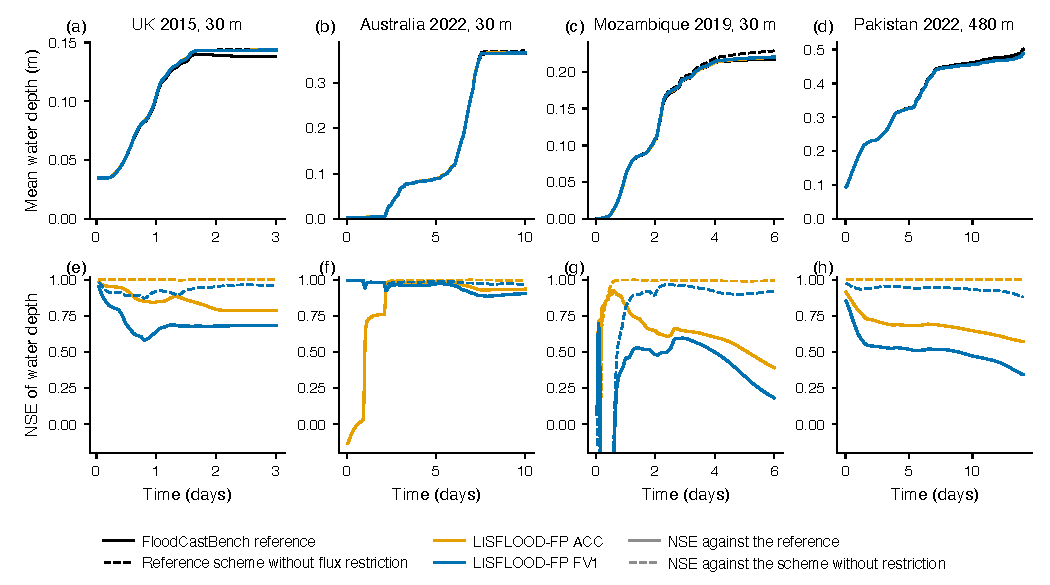
\includegraphics[width=\textwidth]{../figures/f2_floodcastbench.pdf}
\caption{LISFLOOD-FP 8.4 against the FloodCastBench reference simulations.
(a--d) Mean water depth over the domain; (e--h) NSE of the water depth
against the reference (solid) and against the reference scheme without its
flux restriction (dashed).}
\label{fig:fcb}
\end{figure}

The stored water of every run ends within 4.4\,\% of the reference
(Fig.~\ref{fig:fcb}a--d; Table~\ref{tab:fcb}). Against the scheme that
generated the references, run without the flux restriction, the
local-inertial solver of LISFLOOD-FP (ACC) agrees closely: the NSE of the
depths is 1.00 in the UK and Pakistan, 0.96 in Mozambique and 0.87 in
Australia, and the CSI of the flood extent is 0.94--0.98
(Fig.~\ref{fig:fcb}e--h, dashed). The Australian and Mozambican domains are
almost dry for the first two days, when small differences in shallow water
dominate the measure; from the third day on, the NSE of ACC averages 0.99 in
both, against a mean over the whole event of 0.87 (Australia) and 0.96
(Mozambique).
The first-order finite-volume solver (FV1), which solves the full shallow-water
equations rather than the local-inertial approximation, agrees less closely,
with NSE 0.67--0.98 and CSI 0.77--0.94; as the reference scheme and ACC solve
the same approximation, these differences measure the gap between the two
sets of equations on these domains rather than an error of either solver.

Against the references themselves, the agreement is limited by the flux
restriction rather than by the solvers. In Australia, where the restriction
changes the reference little, both solvers reproduce it closely: NSE 0.84
(ACC) and 0.94 (FV1), CSI 0.93 and 0.91. In the UK, ACC reaches an NSE of
0.85 against the reference, which is what the unrestricted scheme itself
achieves (0.86). In Mozambique and Pakistan the restriction matters
more: ACC agrees with the references with NSE 0.63 and 0.68, again
close to the unrestricted scheme (0.67 and 0.67), and the agreement falls
with time as the restricted flow accumulates (Fig.~\ref{fig:fcb}g, h). The
FloodCastBench references are therefore a reproducible benchmark for the
volume and the broad extent of flooding, but their depths in Mozambique and
Pakistan reflect the flux restriction of the generating code. The dataset
contains no infiltration or evaporation, so the loss models are evaluated
against observations in the next section, with CUDA FV1 alone, against three
other first-order finite-volume CUDA solvers and their own loss models.

\subsection{Infiltration: the July 2021 flood of the upper Alzette}\label{sec:alzette}

The simulations of this section use CUDA FV1 on one and four A100 GPUs. The
three codes it is compared with solve the full shallow-water equations with
first-order finite-volume schemes written in CUDA, each with its own
infiltration model, so FV1 gives a like-for-like comparison of the loss
models. ACC is not used here: the local-inertial approximation neglects the
convective acceleration, which is not small in rain-driven flow over the
steep valley sides of this catchment, and the comparison would then measure
the approximation rather than the losses, as Sect.~\ref{sec:fcb} shows for
FV1 against a local-inertial reference.

\paragraph{Event and observations} In July 2021, prolonged heavy rain caused
a major flood in the upper Alzette basin in Luxembourg. The basin covers
467.7\,km$^2$ on a 10\,m grid (4.7 million cells with data in a raster of
4362$\times$2440), with bridge decks removed from the terrain and a gridded
Manning coefficient. Simulations start on 13 July 2021 at 18:00\,UTC from a
stored water depth and run for 96\,h. The rainfall is the gauge-adjusted
radar product RADCLIM of the Royal Meteorological Institute of Belgium
\citep{Goudenhoofdt2016radclim} at 1\,km and 5\,min, of which
38.7 million m$^3$ fall on the basin, most between hours 16 and 28. The
national water authority observes hourly discharge at four gauges, from the
upstream Livange and Hesperange to Pfaffenthal and Steinsel downstream; its
records, kept in UTC+1, are shifted to UTC. Each simulation is scored over
hours 1--96 at each gauge by three measures. The peak ratio (PR) is the
simulated divided by the observed peak discharge, 1 for a perfect peak. The
Nash--Sutcliffe efficiency (NSE; \citealp{NashSutcliffe1970}) is one minus
the sum of squared errors divided by the variance of the observations: 1 for
a perfect hydrograph, 0 for a simulation no better than the observed mean,
negative below it; the squared errors at the peaks dominate it. The
Kling--Gupta efficiency (KGE; \citealp{Gupta2009kge}) is
$1 - \sqrt{(r - 1)^2 + (\beta - 1)^2 + (\gamma - 1)^2}$, where $r$ is the
correlation, $\beta$ the ratio of the simulated to the observed mean
discharge (the bias) and $\gamma$ the ratio of their coefficients of
variation; it is also 1 for a perfect hydrograph, weights timing, volume and
variability equally, and any value above $-0.41$ improves on the observed
mean \citep{Knoben2019}. Simulated discharge is the integral of the unit
discharge normal to transects across the full wetted valley at each gauge,
because at these flows the 10\,m model routes part of the water beside the
surveyed channel. Scored on the surveyed channel alone, the CUDA FV1 runs of
Table~\ref{tab:alzette} give a mean PR of 0.98 and a mean NSE of 0.75 without
infiltration and 0.60 and 0.34 with Green--Ampt, because the water routed
beside the channel is then not counted (the Horton run was not scored in this
way); the full-valley transects are used throughout. The observed peaks rely
on rating curves extrapolated beyond the gauged range, so peak ratios close
to one lie within their uncertainty.

\begin{table}[t]
\caption{Discharge at the four Alzette gauges, July 2021, 96\,h of radar
rainfall, all solvers on the same inputs in double precision: ratio of
simulated to observed peak discharge (PR) and Nash--Sutcliffe efficiency
(NSE) at each gauge, upstream to downstream, and their means over the four
gauges; mean Kling--Gupta efficiency (KGE) over the four gauges; volume
infiltrated over 96\,h where the solver reports it.}
\label{tab:alzette}
\centering\small
\setlength{\tabcolsep}{3.2pt}
\resizebox{\textwidth}{!}{%
\begin{tabular}{@{}ll rrrrr rrrrr r r@{}}
\toprule
& & \multicolumn{5}{c}{PR} & \multicolumn{5}{c}{NSE} & KGE & Infiltrated \\
\cmidrule(lr){3-7}\cmidrule(lr){8-12}
Infiltration & Solver & Liv. & Hes. & Pfa. & Ste. & Mean & Liv. & Hes. & Pfa. & Ste. & Mean & Mean & (10$^6$\,m$^3$) \\
\midrule
\multirow{4}{*}{None} & LISFLOOD-FP & 2.47 & 1.57 & 1.25 & 1.72 & 1.75 & $-1.01$ & 0.30 & 0.77 & 0.43 & 0.12 & 0.55 & -- \\
 & HiPIMS & 2.69 & 1.49 & 1.24 & 1.71 & 1.78 & $-1.75$ & 0.47 & 0.80 & 0.45 & $-0.01$ & 0.58 & -- \\
 & TRITON & 2.29 & 1.28 & 1.20 & 1.49 & 1.57 & $-0.58$ & 0.57 & 0.81 & 0.68 & 0.37 & 0.53 & -- \\
 & SERGHEI-SWE & 2.29 & 1.29 & 1.21 & 1.50 & 1.57 & $-0.60$ & 0.58 & 0.81 & 0.68 & 0.37 & 0.55 & -- \\
\midrule
\multirow{2}{*}{Green--Ampt} & LISFLOOD-FP & 1.14 & 0.79 & 0.78 & 1.12 & 0.95 & 0.72 & 0.67 & 0.57 & 0.68 & 0.66 & 0.46 & 14.1 \\
 & HiPIMS & 1.26 & 0.79 & 0.77 & 1.11 & 0.98 & 0.82 & 0.72 & 0.61 & 0.70 & 0.71 & 0.62 & --$^{a}$ \\
\midrule
\multirow{2}{*}{Horton} & LISFLOOD-FP & 1.04 & 0.74 & 0.75 & 1.08 & 0.90 & 0.73 & 0.64 & 0.53 & 0.65 & 0.64 & 0.46 & 14.4 \\
 & SERGHEI-SWE & 1.84 & 1.01 & 0.95 & 1.28 & 1.27 & 0.24 & 0.63 & 0.84 & 0.77 & 0.62 & 0.47 & 6.7 \\
\bottomrule
\end{tabular}}
\\[2pt]\begin{minipage}{\textwidth}\footnotesize $^{a}$ HiPIMS writes no infiltration or water-balance output.\end{minipage}
\end{table}

\paragraph{Other solvers and rules of the comparison} To separate the loss
models from the hydraulic solver, and to place the cost of CUDA FV1 among
comparable codes, the event is repeated with three independent, open-source
shallow-water solvers written in CUDA that run on one or several NVIDIA GPUs
and solve the same equations with first-order finite-volume schemes: HiPIMS \citep{Xia2019hipims}, which provides
Green--Ampt; SERGHEI-SWE \citep{CaviedesVoullieme2023serghei}, which provides
Horton; and TRITON \citep{MoralesHernandez2021triton}, without infiltration.
They span the two families of Godunov schemes: LISFLOOD-FP FV1 (HLL) and
HiPIMS (HLLC, \citealp{Xia2017srm}) reconstruct the water depth at the cell
faces to balance the bed slope, whereas TRITON and SERGHEI-SWE solve
augmented Roe problems that contain the bed step. The reconstruction adds
operations at every face \citep{ZhaoLiang2022}, and a Roe solver costs more
than HLL or HLLC \citep{Kesserwani2008}; both bear on the run times reported
below. Every solver receives the
same terrain (cells outside the basin without data), Manning coefficients,
initial depth, soil parameters where it infiltrates, rainfall (as a rate on the 10\,m grid; for TRITON, one runoff
series per distinct series of cells, so that every cell receives its
rainfall) and outlet, the 25\,m section where the Alzette leaves the basin. Each solver represents free outflow in its own way:
LISFLOOD-FP removes the water that reaches cells without data, HiPIMS opens
the outline of the domain, TRITON treats cells without data as sinks, and
SERGHEI-SWE, whose faces to such cells are walls, imposes critical flow on
the outlet cells. All four run in double precision and write hourly
outputs, on NVIDIA A100-SXM4-40GB GPUs of one node with one MPI rank per GPU,
on one and on four GPUs. On four GPUs LISFLOOD-FP, TRITON and SERGHEI-SWE
reproduce their single-GPU discharge exactly; HiPIMS does so to within
0.01\,m$^3$\,s$^{-1}$ without infiltration and, with Green--Ampt, gives the
same peaks to within 0.1\,m$^3$\,s$^{-1}$ but differs by up to
3.3\,m$^3$\,s$^{-1}$ at low flow in the first hours. Each solver runs in its documented default configuration, with no option
tuned for speed; SERGHEI-SWE uses its implicit centred friction option, because
its default friction aborted on this case within the first minute, and exchanges halos through GPU-aware MPI,
which its multi-GPU runs require.
Run time is the wall-clock time of the solver process, including reading the
inputs and writing the outputs, and excluding their conversion between
formats. No parameter of any solver was calibrated.

\paragraph{Soil} The Green--Ampt parameters come from European soil
databases: $K_s$ and the saturated water content of the upper 30\,cm from
EU-SoilHydroGrids \citep{Toth2017soil}, the suction head from the texture
relations of \citet{SaxtonRawls2006}, and the initial moisture from SMAP
\citep{Entekhabi2010smap}. Sealed, alluvial and gleyed soils receive $K_s =
0$; the remaining pervious soils cover 71\,\% of the basin with a mean $K_s$
of 0.76\,mm\,h$^{-1}$. In 781\,504 cells (17\,\% of the basin) the SMAP
moisture exceeds the saturated water content of EU-SoilHydroGrids; there
$\Delta\theta$ is zero and the soil infiltrates at $K_s$ from the start, in
both models. For Horton, the same soil is expressed in Horton's
form: in each cell $f_c = K_s$, the rate both models approach once the soil
is wet, and $f_0$ and $k_H$ are fitted by least squares so that the Horton
curve of infiltration under ponding matches that of Green--Ampt over the
first 24\,h (median $f_0 = 5.6$\,mm\,h$^{-1}$, median $k_H =
0.125$\,h$^{-1}$). Under ponding, Green--Ampt and Horton then infiltrate 25.0
and 24.8\,mm after 6\,h and 56.7 and 54.3\,mm after 24\,h (means over the
pervious cells), so differences between runs with the two models reflect the
form of the model, not the soil.


\begin{figure}[tp]
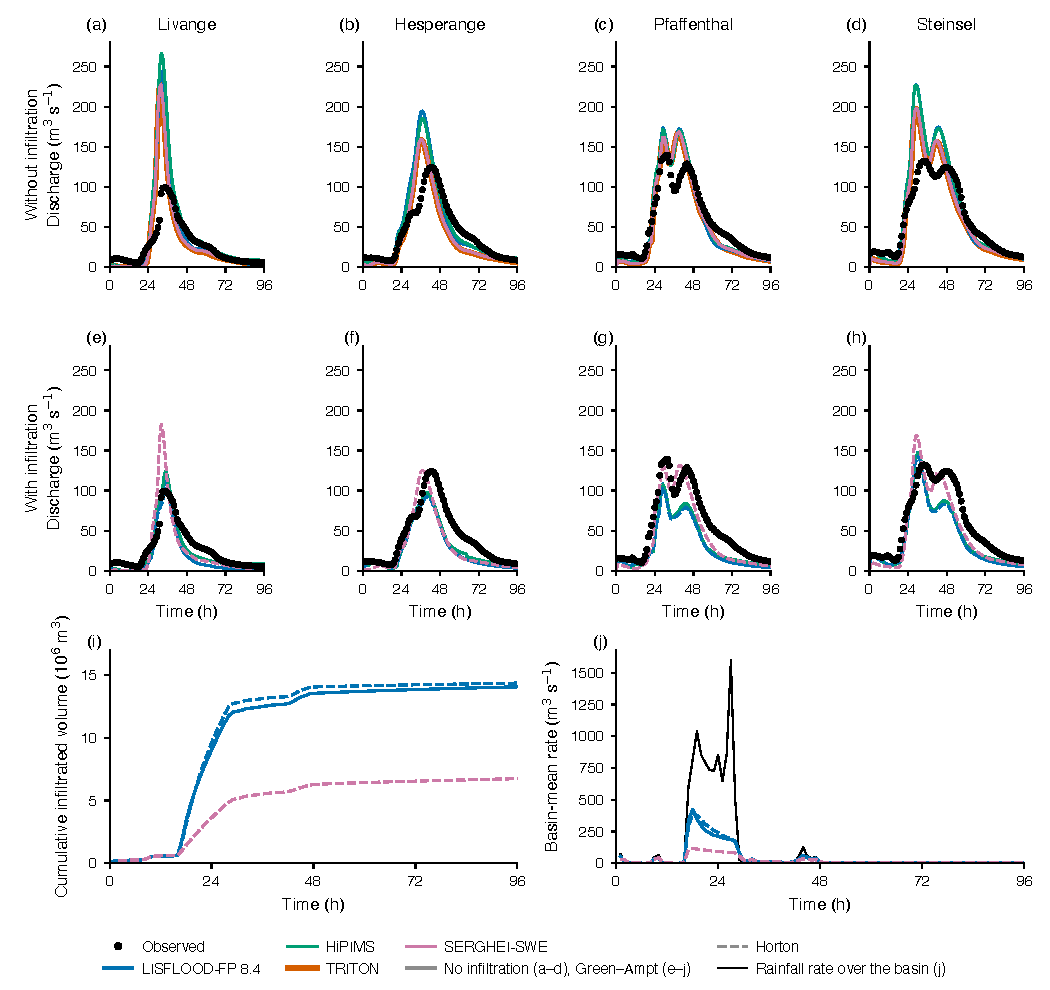
\includegraphics[width=\textwidth]{../figures/f3_alzette.pdf}
\caption{Upper Alzette, July 2021; time in hours since 13 July 2021,
18:00\,UTC. Hourly discharge at the four gauges, upstream to downstream,
observed and simulated: (a--d) without infiltration by the four solvers, (e--h)
with Green--Ampt (LISFLOOD-FP, HiPIMS) and Horton (LISFLOOD-FP, SERGHEI-SWE).
TRITON (wide line) and SERGHEI-SWE coincide in (a--d). (i) Cumulative
volume infiltrated over the basin and (j) its hourly mean rate over the basin,
both in m$^3$\,s$^{-1}$, for the runs that report infiltration: LISFLOOD-FP
with Green--Ampt (blue, solid) and with Horton (blue, dashed), SERGHEI-SWE with
Horton (purple, dashed); HiPIMS writes none. The thin black line in (j) is the
hourly rainfall rate over the basin.}
\label{fig:alzette}
\end{figure}

\paragraph{Hydraulics without infiltration} Without losses every solver
overestimates every peak, by 20--25\,\% at Pfaffenthal and by a factor of
2.3--2.7 at Livange (Table~\ref{tab:alzette}, Fig.~\ref{fig:alzette}a--d), so
the overestimate does not come from one solver. The solvers fall into the two
families of schemes. LISFLOOD-FP and HiPIMS agree with each other (mean PR
1.75 and 1.78), and so do TRITON and SERGHEI-SWE, whose peak discharges
differ by less than 1\,\% (mean PR 1.57). The second family gives lower peaks
at Hesperange and Steinsel, and with them a higher mean NSE (0.37 against
0.12 and $-0.01$), and carries 54--68\,\% of the low flow of the first family
in the first 12\,h at Pfaffenthal and Steinsel (5.8 and 7.6\,m$^3$\,s$^{-1}$,
against 8.6--9.0 and 13.4--14.0\,m$^3$\,s$^{-1}$; observed 14.7 and
18.0\,m$^3$\,s$^{-1}$). LISFLOOD-FP, TRITON and SERGHEI-SWE store and release
nearly the same water: at 96\,h, 15.0--15.8 million m$^3$ remain in the basin
and 24.8--25.5 million m$^3$ have left it, so the schemes differ in how fast
shallow water drains along the valley, not in its volume. No solver represents
baseflow from groundwater: at Livange all carry 0.3--1.2\,m$^3$\,s$^{-1}$ in
the first 12\,h, against 9.1\,m$^3$\,s$^{-1}$ observed.

\paragraph{Green--Ampt run} In LISFLOOD-FP, Green--Ampt removes 14.1 million
m$^3$, 36\,\% of the rain. The outflow falls from 25.5 to 15.5 million m$^3$,
the mean PR from 1.75 to 0.95 and the mean NSE rises from 0.12 to 0.66, with
the largest gain at Livange ($-1.01$ to 0.72; Fig.~\ref{fig:alzette}e--h).
HiPIMS, with its own implementation of the same model, corroborates the
result:
its peak ratios differ from those of LISFLOOD-FP by at most 0.01 at
Hesperange, Pfaffenthal and Steinsel, and its mean NSE is 0.71. The two
differ most at Livange, a wide floodplain gauge where the HiPIMS peak is
11\,\% higher (9\,\% without infiltration). The sensitivity to
the soil is also consistent: halving $K_s$ raises the mean PR to 1.19 in
LISFLOOD-FP and 1.23 in HiPIMS, doubling it lowers the ratio to 0.68 and
0.70, and a wetter initial moisture from ERA5-Land \citep{MunozSabater2021}
raises it to 1.42 and 1.48. Manning coefficients, the initial state and the
rainfall product were not varied, so the uncalibrated scores test the loss
models under one parameterisation, not the best attainable fit. Both solvers
underestimate the recession and the
second peak at Pfaffenthal and Steinsel: infiltrated water leaves the model
for good, whereas in the basin part of it returns to the rivers as subsurface
flow, and the mean simulated discharge there is 56--72\,\% of the observed.
The two efficiencies therefore move in opposite directions: the NSE,
dominated by the peaks, rises, whereas the KGE, which weights the bias in
volume as much as the timing, falls in LISFLOOD-FP from a mean of 0.55 to
0.46, because its bias term $\beta$ drops from 1.0--1.3 at the four gauges
without infiltration to 0.56--0.70 with it. HiPIMS keeps a higher KGE
(0.62), mainly at Livange, where its discharge is closer to the observed
volume.

\paragraph{Horton run and the form of the infiltration model} The Horton run
of LISFLOOD-FP infiltrates 14.4 million m$^3$ (37\,\% of the rain), and its
mean PR and NSE, 0.90 and 0.64, lie within 0.06 and 0.03 of the Green--Ampt
run (Table~\ref{tab:alzette}). With parameters derived from the same soil,
the choice between the two models changes the discharge far less than a
factor of two in $K_s$ does. SERGHEI-SWE, given the same $f_0$, $f_c$ and
$k_H$ in every cell (as 34\,429 parameter classes rounded to four
significant digits), infiltrates only 6.7 million m$^3$, and its peaks are
19--77\,\% higher than those of the LISFLOOD-FP Horton run (mean PR 1.27;
1.84 at Livange, with NSE 0.24).
The shortfall is confined to the loss term: the water SERGHEI-SWE does not
infiltrate leaves the basin (outflow 19.9 against 15.0 million m$^3$) or
remains in it (13.9 against 11.2 million m$^3$), with a closed balance, as
in its run without losses.

SERGHEI-SWE uses Horton's original
equation, $f = f_c + (f_0 - f_c)\,e^{-k_H t}$, with $t$ a clock that every
cell, wet or dry, advances by the time step from the start of the simulation
(\texttt{SourceSink.h} of the version used). LISFLOOD-FP uses the
cumulative form of Sect.~\ref{sec:losses}, in which the capacity falls only
as water infiltrates. In the first 12\,h the rain is lighter than either
capacity, so both solvers infiltrate nearly all of it (0.59 million m$^3$ each). The heavy rain begins about 16\,h after the start; by then the excess
$f - f_c$ of the time-based capacity has decayed to about 14\,\% of $f_0 -
f_c$ at the median $k_H$, also in cells that had stayed dry, whereas the
cumulative capacity of those cells is still $f_0$ and that of the others close
to it. During the storm SERGHEI-SWE therefore infiltrates at 0.3--0.5 of the
rate of LISFLOOD-FP (Fig.~\ref{fig:alzette}j), and by hour 24 it has removed
3.6 against 9.6 million m$^3$ (Fig.~\ref{fig:alzette}i). Applied without flow
to the rainfall of 200\,000 pervious cells with their own parameters, the two
forms alone give the same ratio, 0.38 after 24\,h and 0.42 after 96\,h,
against 0.38 and 0.47 in the simulations, so the difference arises from the
form of the model and not from its parameters or set-up. Parameters fitted to
a ponded infiltration curve assume that the decay starts when ponding starts;
the time-based form starts it at the beginning of the simulation, so its
losses depend on when the simulation starts rather than on the water the soil
has received. The cumulative form removes this dependence, and under it the
Horton and Green--Ampt runs of LISFLOOD-FP agree, as the fit intends. A
fairer test of the time-based form, a run started at the onset of the storm
or parameters refitted to it, was not made; neither would describe the same
soil as the Green--Ampt run. That SERGHEI-SWE reaches a similar mean NSE
(0.62) with higher peaks reflects the lower low flows of its scheme family
(see the hydraulics without infiltration above) rather than a better match
of the losses.

\begin{table}[t]
\caption{Wall-clock time of the 96\,h Alzette simulation in double
precision on NVIDIA A100-SXM4-40GB GPUs of one node, one MPI rank per GPU,
from the start to the end of the solver process; number of time steps.}
\label{tab:modeltimes}
\centering\small
\resizebox{\textwidth}{!}{%
\begin{tabular}{@{}llrrrr@{}}
\toprule
Solver & Infiltration & 1 GPU (min) & 4 GPUs (min) & Speed-up & Steps \\
\midrule
LISFLOOD-FP 8.4 & none & 33.4 & 23.7 & 1.41 & 666\,556 \\
 & Green--Ampt & 33.5 & 24.1 & 1.39 & 661\,820 \\
 & Horton & 34.2 & 24.7 & 1.39 & 662\,612 \\
HiPIMS & none & 250.2$^{a}$ & 80.1 & 3.12 & 1\,726\,457 \\
 & Green--Ampt & 217.2 & 75.0 & 2.89 & 1\,767\,888 \\
TRITON & none & 36.4 & 13.4 & 2.72 & 667\,662 \\
SERGHEI-SWE & none & 59.7 & 50.1 & 1.19 & 935\,374 \\
 & Horton & 62.7 & 47.1 & 1.33 & 930\,337 \\
\bottomrule
\end{tabular}}
\\[2pt]{\footnotesize $^{a}$ Elapsed time of the batch job, which also
queried the GPU; all other times are those of the solver process, so this
time and the speed-up of its row are upper bounds.}
\end{table}

\paragraph{Run time} On one GPU, CUDA FV1 of LISFLOOD-FP is the fastest of
the four solvers: 33.4\,min, against 36.4\,min for TRITON, 60--63\,min for SERGHEI-SWE
and 217--250\,min for HiPIMS (Table~\ref{tab:modeltimes}; the 250\,min is
the elapsed time of the batch job, an upper bound), and also the
fastest per step (3.0\,ms, against 3.3, 3.8--4.0 and 7.4--8.7\,ms). This
order is consistent with the cost of the schemes: HLL in LISFLOOD-FP, the
Roe solver of TRITON and SERGHEI-SWE, and the HLLC solver with face
reconstruction of HiPIMS, which also takes 2.6 times as many steps. The
infiltration models add at most 2.4\,\% to the run time of LISFLOOD-FP. On four GPUs TRITON is fastest
(13.4\,min) and LISFLOOD-FP second (23.7--24.7\,min); Sect.~\ref{sec:performance}
analyses the modest gain of LISFLOOD-FP from four GPUs.

\section{Computational performance}\label{sec:performance}

\subsection{Optimisations of the CUDA FV1 and ACC solvers}\label{sec:opt}

Version 8.4 optimises the steps of the CUDA FV1 and ACC solvers, the two
solvers used for the real events of Sect.~\ref{sec:validation}. The FV1 step
fuses the cell-wise updates, computes the face fluxes in kernels that march
along strips of rows, and reduces the time step in the same kernel as the
rainfall. The ACC step computes the $x$ and $y$ discharges in one kernel,
fuses the depth update with the copies of the old discharges and the
maximum-depth bookkeeping, and reduces the time step on the device, so that
the host waits for the GPU only when it writes output. In both solvers the
release kernels remain available through an environment variable. The CUDA
FV2 and DG2 kernels keep the structure of 8.2 (8.3 added only synchronisation
barriers, and 8.4 the losses).

CUDA FV1 and ACC are faster in 8.4 than in 8.3 in all seven real cases tested with
no loss keyword, so that both versions compute the same simulation: FV1 on
the rain-on-grid 10\,m Alzette grid over 24\,h from a dry start, and FV1 and
ACC on the UK, Australian and Mozambican FloodCastBench inputs. These solvers
were run with both versions in single precision on one A100, alternating on
the same node, and every output raster of the seven cases is byte-identical
between the two versions. Version 8.4 takes 0.30--0.78 of the time of 8.3,
that is, it is 1.3--3.3 times faster, for example 2.0 against 5.5\,min for
FV1 on the Alzette grid (24\,h from a dry start, a different run from those
of Sect.~\ref{sec:scaling}) and 0.18 against 0.51\,min for the UK event with
FV1.

\subsection{Apple Metal against CUDA solvers}\label{sec:metaltime}

Table~\ref{tab:metaltime} compares the four solvers on the two back ends
for the two largest test cases, the torrential valley flood T06 and the
fluvial flood T07s, on one A100 and on the GPU of an Apple M1 Max laptop (32 cores, 400\,GB\,s$^{-1}$ of memory bandwidth against
1555\,GB\,s$^{-1}$). For FV1 the A100 is 3.7--3.9 times faster, in
proportion to the bandwidth of the two devices (3.9), as expected for kernels
bound by memory traffic (Sect.~\ref{sec:roofline}). For ACC it is 6.8--7.8
times faster: the CUDA ACC step was fused in 8.4 (Sect.~\ref{sec:opt}),
whereas the Metal ACC kernels follow the CPU solver (Sect.~\ref{sec:metal}).
For FV2 and DG2 the laptop is
2.5--5.4 times faster than the A100: the CUDA FV2 and DG2 kernels keep the
unoptimised structure of 8.2 (Sect.~\ref{sec:opt}), whereas the Metal
solvers were written for 8.4
with the structure of the 8.3 Metal FV1 (one shared flux per face,
Sect.~\ref{sec:metal}). Their step counts agree to within 0.3\,\%, so the
difference lies in the cost of a step, not in the number of steps. Carrying
the FV1 kernel structure to CUDA FV2 and DG2 is therefore the largest
remaining gain in the CUDA back end.

\begin{table}[t]
\centering\small
\caption{Wall-clock time of the solver process (reading, simulation, writing)
for the same case and solver on one NVIDIA A100 (CUDA) and on an Apple M1
Max (Metal), single precision; time per step in milliseconds; ratio of the M1
Max time to the A100 time. Steps: A100 (M1 Max within 0.3\,\%). T06:
Environment Agency test 5, torrential valley flood, 1.7 million cells, 30\,h.
T07s: Carlisle 2005, fluvial flood, 0.58 million cells, first 6\,h. CUDA ACC
and FV1 are the solvers optimised in 8.4; CUDA FV2 and DG2 keep the
unoptimised kernels of 8.2 (Sect.~\ref{sec:opt}).}
\label{tab:metaltime}
\resizebox{\textwidth}{!}{%
\begin{tabular}{@{}llrrrrrr@{}}
\toprule
& & \multicolumn{2}{c}{A100} & \multicolumn{2}{c}{M1 Max} & & \\
\cmidrule(lr){3-4}\cmidrule(lr){5-6}
Case & Solver & min & ms\,step$^{-1}$ & min & ms\,step$^{-1}$ & Steps & M1 Max\,/\,A100 \\
\midrule
T06 & ACC & 0.5 & 0.19 & 3.3 & 1.27 & 154\,090 & 6.8 \\
 & FV1 & 0.8 & 0.32 & 3.1 & 1.16 & 158\,477 & 3.7 \\
 & FV2 & 45.8 & 11.9 & 8.5 & 2.22 & 230\,264 & 0.19 \\
 & DG2 & 53.3 & 12.2 & 16.6 & 3.79 & 262\,584 & 0.31 \\
T07s & ACC & 0.1 & 0.13 & 0.7 & 1.03 & 37\,886 & 7.8 \\
 & FV1 & 0.2 & 0.20 & 0.8 & 0.78 & 60\,611 & 3.9 \\
 & FV2 & 6.6 & 4.30 & 1.9 & 1.27 & 91\,685 & 0.29 \\
 & DG2 & 14.9 & 4.56 & 6.0 & 1.81 & 196\,409 & 0.40 \\
\bottomrule
\end{tabular}}
\end{table}

\subsection{Scaling of CUDA FV1 on several GPUs for the Alzette basin}\label{sec:scaling}

The scaling of CUDA FV1 was measured on the 10\,m grid of the basin
(10.6 million cells, 4.7 million with data) and on a 5\,m grid of its upper
part (33.9 million cells, 14.4 million with data), over 24\,h and 96\,h,
without infiltration and in single precision; each pair of runs on one and
four A100 GPUs ran consecutively on one node. These simulations are not
those of Sect.~\ref{sec:alzette}: they were set up for the multi-GPU tests,
before the validation runs, with rainfall from the Weather Research and
Forecasting model at 1.3\,km instead of the radar product, and they measure the cost of a step, not the
discharge. The 10\,m simulation over 24\,h restarts from a stored state at
18:00\,UTC on 13 July and the others start dry at 00:00\,UTC on 13 July.

\begin{table}[t]
\centering\small
\caption{Wall-clock time of CUDA FV1 on the Alzette basin, single precision,
NVIDIA A100 GPUs, without infiltration. 10\,m grid: 10.6 million cells,
4.7 million with data; 5\,m grid: 33.9 million cells, 14.4 million with data.
Restart: from a stored state. Efficiency is the speed-up divided by four. All
saved grids are identical on one and four GPUs.}
\label{tab:scaling}
\begin{tabular}{@{}lrrrr@{}}
\toprule
Case & 1 GPU (min) & 4 GPUs (min) & Speed-up & Efficiency \\
\midrule
10\,m, 24\,h (restart) & 4.62 & 3.82 & 1.21 & 30\,\% \\
10\,m, 96\,h & 10.77 & 6.51 & 1.66 & 41\,\% \\
5\,m, 24\,h & 9.79 & 5.64 & 1.74 & 43\,\% \\
5\,m, 96\,h & 55.35 & 28.97 & 1.91 & 48\,\% \\
\bottomrule
\end{tabular}
\end{table}

\begin{figure}[tp]
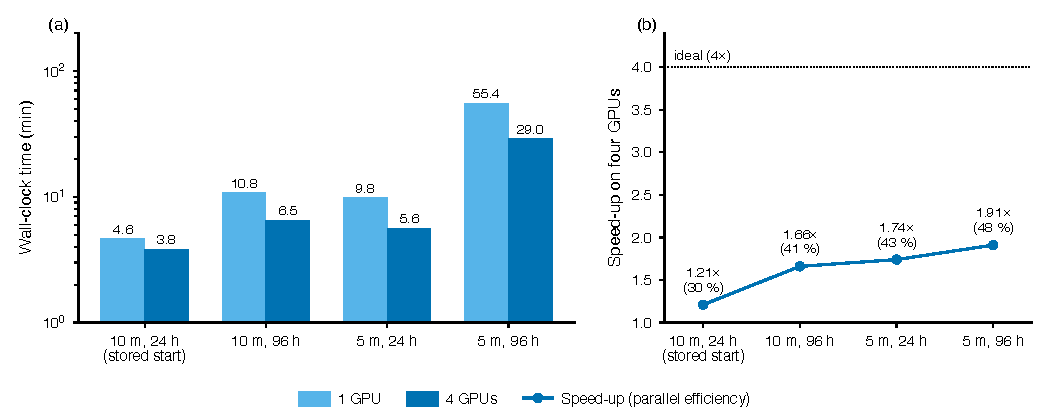
\includegraphics[width=\textwidth]{../figures/f4_scaling.pdf}
\caption{CUDA FV1 on one and four A100 GPUs, Alzette basin, single precision;
10\,m grid: 10.6 million cells, 4.7 million with data; 5\,m grid: 33.9
million cells, 14.4 million with data. (a) Wall-clock time (logarithmic
axis) and (b) speed-up on four GPUs with the parallel efficiency in
parentheses; the dotted line marks ideal scaling.}
\label{fig:scaling}
\end{figure}

Four GPUs shorten the simulations by a factor of 1.21--1.91
(Table~\ref{tab:scaling}, Fig.~\ref{fig:scaling}). The efficiency rises with
the size of the grid and the length of the simulation, from 30\,\% to 48\,\%,
but stays below one half for two reasons. First, a step of 8.4 on one GPU is
short: over the 96\,h simulations (628\,907 and 1\,266\,801 steps) it takes,
in wall-clock time,
1.0\,ms on the 10\,m grid and 2.6\,ms on the 5\,m grid, so the fixed cost of
each step on several GPUs, the exchange of the halo rows through host memory
and the global reduction of the time step, weighs heavily: on four GPUs a
step still takes 0.62 and 1.37\,ms. Second, the ranks own equal bands of
rows, but the wet cells, where the kernels do most of their work, are
unevenly distributed among them, as the profiles below show.

\subsection{Roofline analysis from hardware counters}\label{sec:roofline}

We profiled the three kernels that carry the work of the CUDA FV1 step
(friction and the fluxes and updates across the $x$ and $y$ faces; 2.4\,ms of
the mean step of 3.0\,ms on one GPU at 10\,m) with Nsight Compute 2024.3 and
placed them on a roofline \citep{Williams2009roofline}. The double-precision
build ran the 10\,m Alzette simulation of Sect.~\ref{sec:alzette} and the
5\,m simulation of Table~\ref{tab:scaling}, and sixteen consecutive launches
of each kernel were replayed and averaged at a wet state: hour 30 of the
10\,m case, during the flood, and hour 24 of the 5\,m case. On four GPUs the
launches of the same steps were profiled on every rank. Performance counts the
FP64 additions, multiplications and fused multiply--adds (two operations
each); the arithmetic intensity divides it by the traffic to device memory
(DRAM). The profiles describe double precision, in which a 10\,m step takes
3.0\,ms (Table~\ref{tab:modeltimes}); the single-precision steps of
Table~\ref{tab:scaling} are about three times shorter, with other rainfall
and start, so the profiles illustrate rather than measure the balance of that
table.

\begin{table}[t]
\centering\small
\caption{Roofline metrics of the three kernels of the CUDA FV1 step on the
A100, double precision, means over 16 launches at a wet state. AI: arithmetic
intensity (FLOP\,byte$^{-1}$); GFLOP\,s$^{-1}$: FP64 performance; DRAM and
L2: throughput as a percentage of the peak (DRAM 1555\,GB\,s$^{-1}$). Four
GPUs: range of the DRAM throughput over the ranks.}
\label{tab:roofline}
\setlength{\tabcolsep}{3.5pt}
\resizebox{\textwidth}{!}{%
\begin{tabular}{@{}l rrrr rrrr rr@{}}
\toprule
& \multicolumn{4}{c}{10\,m, 1 GPU} & \multicolumn{4}{c}{5\,m, 1 GPU} & \multicolumn{2}{c}{4 GPUs, DRAM} \\
\cmidrule(lr){2-5}\cmidrule(lr){6-9}\cmidrule(l){10-11}
Kernel & AI & GFLOP\,s$^{-1}$ & DRAM & L2 & AI & GFLOP\,s$^{-1}$ & DRAM & L2 & 10\,m & 5\,m \\
\midrule
Friction & 0.42 & 344 & 52 & 68 & 0.31 & 262 & 54 & 62 & 29--51 & 32--54 \\
Flux, $x$ faces & 1.75 & 1238 & 45 & 70 & 1.50 & 1234 & 53 & 76 & 7--31 & 27--49 \\
Flux, $y$ faces & 0.92 & 786 & 55 & 70 & 0.80 & 770 & 62 & 73 & 13--44 & 40--60 \\
\bottomrule
\end{tabular}}
\end{table}

\begin{figure}[tp]
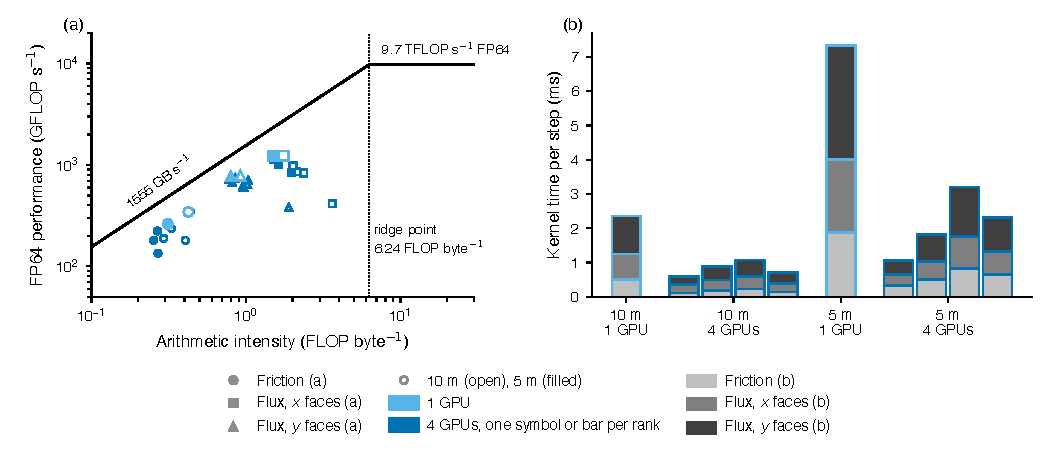
\includegraphics[width=\textwidth]{../figures/f5_roofline.pdf}
\caption{The kernels of the CUDA FV1 step on the A100, double precision;
10\,m grid: 10.6 million cells, 4.7 million with data; 5\,m grid: 33.9
million cells, 14.4 million with data. (a) Roofline: FP64 performance against
arithmetic intensity (filled symbols 5\,m, open 10\,m); the dotted line marks the ridge point between kernels limited by memory bandwidth and by
arithmetic. (b) Time of the three kernels in one step on each GPU: one GPU,
and each rank of four.}
\label{fig:roofline}
\end{figure}

The ridge point of the A100 in double precision lies at 6.24\,FLOP\,byte$^{-1}$
(9.7\,TFLOP\,s$^{-1}$ divided by 1555\,GB\,s$^{-1}$). On one GPU the three
kernels reach 0.3--1.8\,FLOP\,byte$^{-1}$ and at most 13\,\% of the FP64 peak,
and on four GPUs at most 3.6\,FLOP\,byte$^{-1}$ (Table~\ref{tab:roofline},
Fig.~\ref{fig:roofline}a), so their speed is set by memory traffic rather
than arithmetic. On one GPU they use 45--62\,\% of the DRAM bandwidth and
62--76\,\% of the L2 bandwidth: the fused kernels take much of their data from
the cache, and the metrics hardly change between the two grids. On four GPUs
the ranks differ (Fig.~\ref{fig:roofline}b). The kernels of the busiest rank
take 1.07\,ms per step at 10\,m and 3.20\,ms at 5\,m, against 2.36 and
7.33\,ms on one GPU, so that even with free communication four GPUs could
run the kernels only 2.2--2.3 times faster. Balancing the ranks by wet cells
rather than rows, and exchanging halos directly between GPUs, are therefore
the most promising routes to better scaling, and reducing the memory traffic
per cell the route to faster steps.

\section{Limitations}\label{sec:limits}

Neither infiltration model lets the soil drain and regain capacity between
rain events (Sect.~\ref{sec:losses}), so both suit single events; long
simulations require such a recovery, or an initial moisture from a
hydrological model.
Evaporation is uniform in space and was verified against analytical
solutions only; the FloodCastBench and Alzette simulations apply no
evaporation. The Horton parameters of the Alzette basin were derived from the
Green--Ampt soil, not measured.

The dense Metal modes (Sect.~\ref{sec:metal}) provide no non-uniform or
adaptive mesh. A six-hour Alzette matrix of 28 runs at 100\,m, the seven
solver keywords with each loss option, completed on Metal, but the
adaptive-grid CUDA solvers were not validated on the basin and are not
suited to rain-on-grid simulation: CUDA MWDG2 reads no rainfall input and
stalled after 11.37\,s with a time step below the resolution of its
single-precision clock, and CUDA HWFV1 ignores the dynamic rainfall file and
wrote small negative depths.

CUDA FV2 and DG2 on several GPUs reproduce the single-GPU water balance but
are fast only when each rank sees only its own GPU (a wrapper script is
provided); their device binding has not yet been optimised, and their scaling
on full workloads has not been measured. All Metal results come from one
Apple M1 Max laptop, whose single 32-core GPU shares 64\,GB of memory with the CPU.
The row decomposition of Sect.~\ref{sec:multigpu} runs on Metal with several
ranks and was verified with two (Sect.~\ref{sec:gputests}), but every rank
opens the default device, so a computer with several Metal GPUs was not
tested. The \texttt{.mass} diagnostics of Metal runs
with several ranks are not yet correct, although their depth rasters are.
The row partition and the halo exchange through host memory limit the scaling
of FV1 (Sect.~\ref{sec:roofline}), and the CUDA FV2 and DG2 kernels, which
keep the structure of 8.2, take 4--12\,ms per step where the Metal ports take
1--4 (Sect.~\ref{sec:metaltime}).

CUDA FV2 and DG2 keep the bed elevation in single precision as given
(Sect.~\ref{sec:losstests}). The following behaviours of the 8.3 solvers were
found while porting and are reported rather than changed: CUDA and Metal DG2
become unstable on T07 after about 4\,h and write negative depths on T06;
CUDA ACC, whose results 8.4 does not change, is unstable on T05 (CPU and CUDA
agree on 6\,\% of wet cells) and became unstable with evaporation on the
100\,m Alzette matrix above, where Metal ACC stayed bounded; on the plane of
Sect.~\ref{sec:freetest}, where no water may cross the free edge, the free
boundaries of CUDA ACC and HWFV1, which 8.4 does not change, lose 1.5\,\% and
21\,\% of the volume in 30\,min (DG2 and MWDG2 0.05\,\%); the CUDA FV2
slope limiter evaluates minus the inverse of the usual ratio (e.g.
\citealp{Ayog2021}), so it returns a zero slope on
monotone profiles and a non-zero slope only at local extrema, where a limiter
should return zero; and CUDA applies dynamic rain
and point sources with the time step of the previous step. One defect was
corrected: CUDA ACC did not wait for its last output before freeing memory (a
call commented out in 8.2), which truncated the last output in one run of
T03.

\section{Conclusions}\label{sec:conclusions}

LISFLOOD-FP 8.4 makes rainfall losses part of every GPU simulation, on CUDA
and on Apple Metal, distributes the uniform-grid FV1, FV2 and DG2 over
several GPUs and runs the uniform-grid FV1 and ACC 1.3--3.3 times faster
than 8.3 (Table~\ref{tab:support}).

Verification shows that the loss models reproduce analytical solutions to
within 1\,mm on every solver and both back ends, that a run of 8.4 with no
loss keyword reproduces 8.3 exactly, and that CUDA FV1 gives identical results on one and four
GPUs. On the
FloodCastBench events, set up as the published code that generated the
references, LISFLOOD-FP 8.4 ends within 4.4\,\% of the reference volume, and
its local-inertial solver agrees with the generating scheme with an NSE of
0.87--1.00 once that scheme's restriction to eastward and southward flow is
removed.

For the July 2021 flood of the upper Alzette, run with CUDA FV1 and three
independent first-order finite-volume CUDA solvers on the same inputs,
precision and hardware, every solver overestimates the peaks without
infiltration, so the losses are needed whatever the
hydraulic scheme. Green--Ampt infiltration parameterised from European soil
data without calibration removes 36\,\% of the rain and raises the mean NSE
of discharge at four gauges from 0.12 to 0.66, in close agreement with HiPIMS
(0.71). A Horton parameterisation of the same soil gives 0.64. The time-based
Horton model of SERGHEI-SWE, with the same parameters, infiltrates half as
much, because its capacity decays before the storm whether or not the soil
has received water; the cumulative form of 8.4 removes this dependence on the
start of the simulation. On one A100 GPU, CUDA FV1 completes the
simulation of 4.7 million cells with data in 33\,min, the fastest of the
four solvers.
Its kernels are bound by memory bandwidth and its single-GPU step is short,
so on four GPUs the uneven wet area of the row partitions and the fixed cost
of each step limit the speed-up to 1.2--1.9; balancing the partitions by wet
cells and exchanging halos directly between GPUs are the next steps, together
with the implementation of the FV1 kernel structure in CUDA FV2 and DG2,
which the Metal ports already have (Sect.~\ref{sec:metaltime}).


\section*{Software and data availability}
\textit{Name of software}: LISFLOOD-FP 8.4. \textit{Developer and contact}:
Haseeb ur Rehman, University of Luxembourg, haseeb.rehman@uni.lu; LISFLOOD-FP
is developed by the universities of Bristol, Sheffield and their collaborators
since 1999. \textit{Year first available}: 2026 (version 8.4). \textit{Hardware
required}: an NVIDIA GPU (CUDA 11.4 or later) or an Apple Silicon Mac; several
NVIDIA GPUs with MPI for the multi-GPU runs; a CPU build is also provided.
\textit{Software required}: CMake 3.13 or later, a C++ compiler, the CUDA
toolkit or Xcode, NetCDF-C, OpenMP and libnuma on Linux, MPI optional.
\textit{Program language}: C++, CUDA and the Metal Shading Language.
\textit{Program size}: about 200\,000 lines of source; the source archive with
the tests and the example is 75\,MB. \textit{Availability and cost}: free and
open source under the GNU General Public License v3. The source of LISFLOOD-FP
8.4, the patch from 8.3, the tests of Sect.~\ref{sec:verification}, the scripts
that set up the FloodCastBench and Alzette simulations and that re-run the
FloodCastBench generation code, and the data and scripts behind the tables and
figures are archived at Zenodo (\url{https://doi.org/10.5281/zenodo.24098586}). FloodCastBench is available from
\citet{Xu2025floodcastbench}. The Alzette inputs (Sect.~\ref{sec:alzette})
are part of the archive; the observed discharge was provided by
the Administration de la gestion de l'eau of Luxembourg. The comparison of
Sect.~\ref{sec:alzette} used HiPIMS (\url{github.com/HEMLab/HiPIMS-CUDA},
commit 0a27363), SERGHEI-SWE (\url{gitlab.com/serghei-model/serghei}, commit
2728883) and TRITON (\url{github.com/lassiterdc/triton}, commit a57ce39); the
scripts that convert the inputs for them and score all runs are part of the
archive.

\section*{CRediT authorship contribution statement}
\textbf{Haseeb ur Rehman}: Conceptualization, Methodology, Software,
Investigation, Formal analysis, Visualization, Writing -- original draft.
\textbf{F\'{e}licia Norma Teferle}: Supervision, Funding acquisition,
Writing -- review \& editing. \textbf{Georges Kesserwani}: Conceptualization,
Writing -- review \& editing.

\section*{Declaration of competing interest}
The authors declare that they have no known competing financial interests or
personal relationships that could have appeared to influence the work reported
in this paper.

\section*{Acknowledgements}
Funding: This work was supported by the Fonds National de la Recherche
Luxembourg (FNR) under the Industrial Fellowship (IF) grant [project number
17130773].

\section*{Declaration of generative AI and AI-assisted technologies in the manuscript preparation process}
During the preparation of this work the authors used Anthropic's Claude
models (Opus 5.5 and Fable 5.1) to improve the grammar and language of the
manuscript and for AI-assisted coding and debugging of parts of the CUDA and Metal
code. After using this tool, the authors reviewed and edited the content as
needed and take full responsibility for the content of the published article.

\bibliographystyle{elsarticle-harv}
\bibliography{references}

\end{document}
